\documentclass[a4paper,11pt,reqno]{amsart}
\usepackage{M67}

\DeclareMathOperator{\aire}{aire}

\begin{document}

\hautdepage{TD3: Géométrie plane}

\vspace{-3mm}
\begin{convention}
  On se place dans le plan $\ens{P}=\R^2$.
\end{convention}

% ==================================
\section{Propriétés basiques -- Cours}
% ==================================


%-----------------------------------
\begin{exo}[.35]

  Montrer que deux droites perpendiculaires à une troisième sont parallèles.
\end{exo}

%-----------------------------------
\begin{exo}[.49] (Médiatrice)

  Soient $A$ et $B$ deux points distincts. Montrer que l'ensemble des points $M$ tels que $AM=BM$ est la droite perpendiculaire à $(AB)$ passant par le milieu de $[AB]$.
\end{exo}

%-----------------------------------
\begin{exo} (Bissectrice et longueurs)

  Soit $M$ le pied de la bissectrice issue de $A$ dans un triangle $\tri ABC$ (c.-à-d. le point d'intersection de cette bissectrice et du côté opposé $[BC]$).
  \begin{enumerate}
    \item Montrer l'égalité des rapports $AB:AC=MB:MC$.
    \item Montrer que la bissectrice $AM$ coupe le cercle circonscrit en un point $P$ qui est sur la médiatrice de $[BC]$.
    \item Montrer que $AM^{2} = AB \times AC - MB \times MC$
  \end{enumerate}
\end{exo}

%-----------------------------------
\begin{exo} (Parallélogrammes) % parallelogrammes : cotes paralleles deux a deux ; quadrilateres : 4 segments

  \begin{enumerate}
    \item On dit que quadrilatère $ABCD$ est \emph{convexe} s'il est \emph{non dégénéré} (sans trois sommets alignés), \emph{non croisé} (les intérieurs des côtés (opposés) ne se rencontrent pas) et sans sommet à l'intérieur du triangle formé par les trois autres. Montrer qu'un quadrilatère $ABCD$ est convexe si et seulement si les \emph{diagonales} $[AC]$ et $[BD]$ se rencontrent.
    \item Montrer que pour un quadrilatère convexe $ABCD$ les conditions suivantes sont équivalentes :
    \begin{enumerate}
      \item c'est un parallélogramme ;
      \item les angles opposés sont égaux ;
      \item les côtés opposés sont égaux ;
      \item deux côtés opposés sont parallèles et égaux ;
      \item ses diagonales $[AC]$ et $[BD]$ se coupent en leur milieu.
    \end{enumerate}
    \item Montrer qu'un parallélogramme est un rectangle (resp. un losange) si et seulement si ses diagonales sont égales (resp. perpendiculaires).
    \item Montrer que les bissectrices d'un parallélogramme forment un rectangle. À quelle condition forment-elles un carré ?
    \item Montrer que les milieux des côtés d'un quadrilatère (convexe) sont les sommets d'un parallélogramme.
  \end{enumerate}
\end{exo}

%-----------------------------------
%-----------------------------------
\begin{exo} (Quadrilatère inscrit)

    Soit $ABCD$ un quadrilatère non croisé.
    \begin{enumerate}
      \item Montrer que si $ABCD$ est inscrit dans un cercle, alors $ABCD$ est convexe (et ses diagonales se coupent en un point).
      \item Montrer l'équivalence des assertions suivantes:
      \begin{enumerate}
        \item $ABCD$ est inscrit dans un cercle.
        \item $ABCD$ est convexe et $\widehat{ABC}+\widehat{CDA} = \pi$ (ou $\widehat{DAB}+\widehat{BCD} = \pi$).
        \item $[AC]$ et $[BD]$ se coupent en $S$ et $AS \times SC = BS \times SD$.
        \item $AB\times CD + BC\times DA = AC\times BD$ (c'est le \emph{théorème de Ptolémée}).
      \end{enumerate}
    \end{enumerate}
\end{exo}

%-----------------------------------
\begin{exo} (Cas de similitude)

  Soient $\tri ABC$ et $A'B'C'$ deux triangles non dégénérés et non confondus, tels que $(A'B') \parallel (AB)$, $(A'C') \parallel (AC)$ et $(B'C') \parallel (BC)$.
  \begin{enumerate}
    \item Montrer que les triangles $\tri ABC$ et $A'B'C'$ sont semblables.
    \item Montrer que de plus les droites $(AA')$, $(BB')$ et $(CC')$ sont parallèles ou concourantes.
  \end{enumerate}

\end{exo}


%-----------------------------------
\begin{exo} (Points remarquables dans le triangle)

  Soit $\tri ABC$ un triangle non dégénéré.
  \begin{enumerate}
    \item Montrer que les trois bissectrices sont concourantes. Montrer que leur point commun est centre d'un \emph{cercle inscrit} dans le triangle $\tri ABC$, et qu'il n'y a qu'un seul tel centre (et un seul tel cercle).
    \item Montrer que la bissectrice d'un angle et les bissectrices extérieures des deux autres angles sont également concourantes.
    \item Montrer que les trois médiatrices du triangle sont concourantes. Montrer que leur point commun est \emph{centre du cercle circonscrit} au triangle $\tri ABC$.
    \item Montrer que les trois médianes sont concourantes en un point situé au tiers de chacune d'elles en partant de la base correspondante. On appelle \emph{centre de gravité} ou \emph{barycentre}\footnote{ou \emph{isobarycentre}, ou \emph{centroïde}.} leur point d'intersection.
    \item Montrer que le centre du cercle circonscrit, l'orthocentre et le centre de gravité sont alignés (on appelle \emph{droite d'Euler} la droite passant par ces trois points).
    \item Montrer que les trois hauteurs sont concourantes. On appelle \emph{orthocentre} leur point d'intersection.
  \end{enumerate}
\end{exo}

%-----------------------------------
\begin{exo} (Rayons des cercles circonscrit et inscrit)

  Soit $\tri ABC$ un triangle de longueurs de côtés $a$, $b$ et $c$ et de mesures des angles respectifs $\alpha$, $\beta$ et $\gamma$.
  \begin{enumerate}
    \item Exprimer le rayon $R$ du cercle circonscrit en fonction des longueurs des côtés et des angles du triangle.
    \item Exprimer le rayon $r$ du cercle inscrit en fonction du périmètre et de l'aire du triangle.
    \item Exprimer le rayon $r$ du cercle inscrit en fonction des longueurs des côtés et des angles du triangle.
    \item Exprimer le rapport $\frac{R}{r}$ en fonction des angles du triangle.
  \end{enumerate}
\end{exo}


% ==================================
\section{Dans le triangle}
% ==================================

%-----------------------------------
\begin{exo}[.49]

  Soient $\tri ABC$ un triangle et $H$ son orthocentre. Soit $H'$ le symétrique de $H$ par rapport à $(BC)$ Montrer que $H'$ est sur le cercle circonscrit à $\tri ABC$.
\end{exo}

%-----------------------------------
\begin{exo}[.7]

  Soient $\tri ABC$ un triangle et $P$, $Q$, $R$ trois points situés respectivement sur $[BC]$, $[CA]$ et $[AB]$. Montrer que les cercles circonscrits aux triangles $AQR$, $BRP$ et $CPQ$ ont un point commun.\\
  \begin{indication}
    Attention au cas où deux des cercles se touchent.
  \end{indication}
\end{exo}


%-----------------------------------
\begin{exo} (Carré dans un triangle)

  Soit $\tri ABC$ un triangle \emph{acutangle}\footnote{À angles aigus.}.
  \begin{enumerate}
    \item Montrer qu'il existe un carré $IJKL$ avec $I,J \in [AB]$, $K \in [BC]$ et $L \in [CA]$. En donner une construction.
    \item Un tel carré est-il unique ?
    \item Que se passe-t-il si le triangle a un angle obtus ?
  \end{enumerate}
\end{exo}

%-----------------------------------
\begin{exo} (Inégalité triangulaire)

  Soit $\tri ABC$ un triangle.
  \begin{enumerate}
    \item \label{plusgrand} Montrer que si $AB > AC$, alors $\widehat{C}>\widehat{B}$ (on pourra considérer $B' \in [AB]$ tel que $AB'=AC$). % ou utiliser la loi des sinus
    \item Montrer qu'on a en fait équivalence: $AB>AC$ si et seulement si $\widehat{C}>\widehat{B}$.
    \item En déduire l'inégalité triangulaire: dans un triangle, chacun des côtés est plus petit que la somme des deux autres.
    \item Déduire de la question \ref{plusgrand}) qu'un disque est convexe.
  \end{enumerate}
\end{exo}


%-----------------------------------
\begin{exo}[.7] (Triangle orthique)

  Soit $\tri ABC$ un triangle non rectangle. On note respectivement $H_A$, $H_B$ et $H_C$ les pieds des hauteurs issues de $A$, $B$ et $C$. Montrer que les bissectrices du triangle $\tri H_AH_BH_C$ sont les hauteurs du triangle $\tri ABC$.
\end{exo}

%-----------------------------------
\begin{exo} (Tout triangle est isocèle)

  On donne ici un argument pour établir que tout triangle est isocèle (dû à W.W. Rouse Ball).
  Soit $\tri ABC$ un triangle quelconque. Soit $D$ le point d'intersection de la bissectrice de l'angle $\widehat{BAC}$ avec la médiatrice du côté opposé $[BC]$. Soient $E,F$ et $G$ les projetés orthogonaux de $D$ sur $[BC]$,$[AB]$ et $[AC]$.
  \sidebyside{.70}{
    \begin{enumerate}
      \item Montrer que $DF=DG$ et $AF=AG$.
      \item Montrer que $DB=DC$, puis que $FB=GC$.
      \item En déduire que $\tri ABC$ est isocèle, puis qu'il est équilatéral.
      \item Comment expliquer cela ?
    \end{enumerate}
  }{
    \raisebox{-28mm}[0pt][0pt]{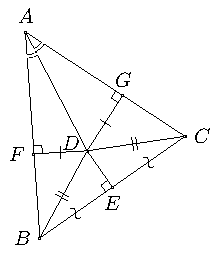
\includegraphics[width=35mm]{img_isocele_ball}}
  }
\end{exo}

% ==================================
\section{Cercles, angles et longueurs}
% ==================================

%-----------------------------------
\begin{exo}

  Soient $A$ et $B$ deux points et $\gamma \in ]0,\pi[$ donnés. Soit $\Gamma$ l'ensemble des points $C$ tels que $\widehat{ACB}=\gamma$.
  \begin{enumerate}
    \item Décrire l'ensemble $\Gamma$. Sous quelle condition $\Gamma$ est un cercle ?
    \item Montrer que quand $C$ parcourt $\Gamma$, l'isobarycentre $G$ de $\tri ABC$ parcourt deux arcs de cercles. Sous quelle condition $G$ parcourt un cercle ?
    \item Montrer que quand $C$ parcourt $\Gamma$, le centre du cercle inscrit $I$ de $\tri ABC$ parcourt deux arcs de cercles. Sous quelle condition $I$ parcourt un cercle ?
    \item Quand $C$ parcourt $\Gamma$, quelle est l'ensemble parcouru par le centre du cercle circonscrit de $\tri ABC$ ?
    \item Montrer que quand $C$ parcourt $\Gamma$, l'orthocentre $H$ de $\tri ABC$ parcourt deux arcs de cercles. Sous quelle condition $H$ parcourt un cercle ?
  \end{enumerate}
\end{exo}

%-----------------------------------
\begin{exo} (Puissance d'un point)

  Soient $M$ un point et $\ens{C}$ un cercle. On considère une droite $\ens{D}$ passant par $P$ et qui rencontre $\ens{C}$ en deux points (pas forcément distincts) $S$ et $T$.
  \begin{enumerate}
    \item Montrer que la quantité $\overline{MS}\times \overline{MT}$ ne dépend pas du choix de la droite $\ens{D}$.
  \end{enumerate}
  \begin{convention}
    Pour la suite on note cette quantité $P_{\ens{C}}(M)$ et on l'appelle \emph{puissance de $M$ par rapport à $\ens{C}$}.
  \end{convention}
  \begin{enumerate}[resume]
    \item Étant donné un cercle $\ens{C}$, déterminer le signe de $P_{\ens{C}}(M)$ en fonction de la position de $M$.
    \item Montrer que l'ensemble des points à égale puissance par rapport à deux cercles non concentriques donnés est une droite (appelée \emph{axe radical} de ces deux cercles).
    \item Déterminer l'axe radical dans le cas de deux cercles distincts qui s'intersectent.
    \item Quelle droite «connue» généralise l'axe radical.
    \item Étant donnés deux cercles non concentriques, construire à la règle et compas l'axe radical.
  \end{enumerate}
\end{exo}

%-----------------------------------
\begin{exo} (Angle entre deux cercles)

  Soient deux cercles $\ens{C}_{1}$ et $\ens{C}_{2}$ de centres respectifs $O_{1}$ et $O_{2}$ qui se rencontrent en un point $S$. On définit (la mesure de) l'angle entre $\ens{C}_{1}$ et $\ens{C}_{2}$ comme étant égale à $\widehat{O_{1}MO_{2}}$.
  \begin{enumerate}
    \item Quelle est l'angle entre deux cercles tangents extérieurement ?
    \item Quelle est l'angle entre deux cercles tangents intérieurement ?
    \item Soient un cercle $\ens{C}$ et un point $M$ extérieur à $\ens{C}$. Montrer qu'il existe un cercle de centre $M$ qui est orthogonal\footnote{Qui fait un angle de $\pi/2$ avec $\ens{C}$.} à $\ens{C}$.
    \item Étant donnés deux cercles, déterminer l'ensemble des centres des cercles orthogonaux à ces deux cercles.
    \item Étant donnés trois cercles en position générale, montrer qu'il existe un unique cercle qui est orthogonal aux trois.
  \end{enumerate}
\end{exo}


% ==================================
\section{Utilisation des aires}
% ==================================

\begin{convention}
  On note $\aire (P)$ l'aire d'une figure $P$.
\end{convention}

%-----------------------------------
\begin{exo}[.35]

  Soit $T$ un triangle inclus dans un rectangle $R$. Montrer que $\aire(T) \leqslant \frac{1}{2}\aire{R}$.
\end{exo}

%-----------------------------------
\begin{exo}
  Soit $\tri ABC$ un triangle inscrit dans le cercle fixé $\ens{C}$.
  \begin{enumerate}
    \item Sous quelle condition l'aire de $\tri ABC$ est maximale ?
    \item Sous quelle condition $AB^{2}+BC^{2}+CA^{2}$ est maximal ?
    \item Et pour un quadrilatère $ABCD$ ?
  \end{enumerate}

\end{exo}

%-----------------------------------
\begin{exo} (Théorèmes de Gergonne et de Céva)

  Soient $\tri ABC$ un triangle et $A'$, $B'$, $C'$ trois points de $(BC)$, $(AC)$ et $(AB)$.
  \begin{enumerate}
    \item Si $(AA')$, $(BB')$ et $(CC')$ sont concourantes en un point $M$ intérieur au triangle $\tri ABC$, alors on a la relation de Gergonne
    $$
      \frac{MA'}{AA'}+\frac{MB'}{BB'}+\frac{MC'}{CC'}=1.
    $$
    \begin{indication}
      Interpréter les rapports comme des rapports d'aires.
    \end{indication}
    \item Les trois droites $(AA')$, $(BB')$ et $(CC')$ sont concourantes si et seulement si la relation de Céva
      $$
        \frac{\overline{A'B}}{\overline{A'C}}\frac{\overline{B'C}}{\overline{B'A}}\frac{\overline{C'A}}{\overline{C'B}}=-1.
      $$
  \end{enumerate}
\end{exo}

%-----------------------------------
\begin{exo} (Formule de Héron)

  \begin{enumerate}
    \item Montrer que l'aire d'un triangle $\tri ABC$ de côtés de longueurs $a$, $b$ et $c$ et de demi-périmètre $p=\frac{1}{2}(a+b+c)$ est
    $$
      \aire{(ABC)}=\sqrt{p(p-a)(p-b)(p-c)}.
    $$
    \begin{indication}
      Exprimer $\sin^2(\widehat{A})$.
    \end{indication}
    \item En déduire une expression du rayon du cercle inscrit en fonction des longueurs des côtés.
  \end{enumerate}
\end{exo}

%-----------------------------------
\begin{exo}[.7] (Longueurs des hauteurs)

  Donnes une condition nécessaire et suffisante sur trois nombres réels $h_{A}$, $h_{B}$ et $h_{C}$ pour qu'ils soient les longueurs des hauteurs d'un triangle.\\
  Et pour qu'ils soient les longueurs des hauteurs d'un triangle acutangle ?
\end{exo}

%-----------------------------------
\begin{exo}[.49] (Partage de trapèze)

  Soit $ABCD$ un trapèze de grande base $CD$ et de petite base $AB$. Construire un point $M$ de $[CD]$ tel que $(AM)$ partage le trapèze en deux parties de même aire.
\end{exo}

%-----------------------------------
\begin{exo}[.35] (Rosace)

  Calculer l'aire de la rosace à 6 feuilles construite au compas.
\end{exo}

%-----------------------------------
\begin{exo}[.49]

  Deux disques $D_1$ et $D_2$ de même rayon $R$ sont tangents extérieurement et tangents, en deux autres points, à une même droite $\Delta$. Calculer l'aire du disque $D$ tangent à la fois à $D_1$, $D_2$ et $\Delta$.
\end{exo}

%-----------------------------------
\begin{exo} (Kangourou 2007)

  \sidebyside{.7}{
    Soient deux demi-cercles tangent intérieurement (en $K$ sur la figure ci-contre). La corde $[MN]$ est parallèle à la droite $(KL)$, contenant les deux centres, et tangente au petit demi-cercle ; elle mesure 4. Combien vaut l'aire (grisée sur la figure) entre les deux demi-cercles ?
  }{
    \raisebox{-21mm}[0pt][0pt]{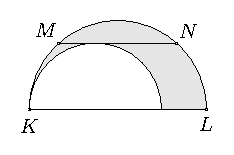
\includegraphics[width=5cm]{img_kangourou2007}}
  }
\end{exo}

%-----------------------------------
\begin{exo}[.7] (Kangourou 2006 et DS2 de 2018)

  \sidebyside{.7}{
    On considère la figure ci-contre ; le quotient du rayon du secteur circulaire par le rayon du cercle inscrit dans ce secteur est 3. Quel est le quotient des aires de ce secteur circulaire et du cercle inscrit ?
  }{
    \raisebox{-21mm}[0pt][0pt]{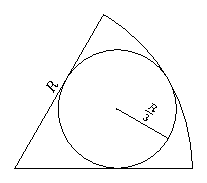
\includegraphics[width=4cm]{img_kangourou2006}}
  }
\end{exo}

\end{document}
